\begin{figure}[ht!]
    \begin{subfigure}{\textwidth}
    \centering
    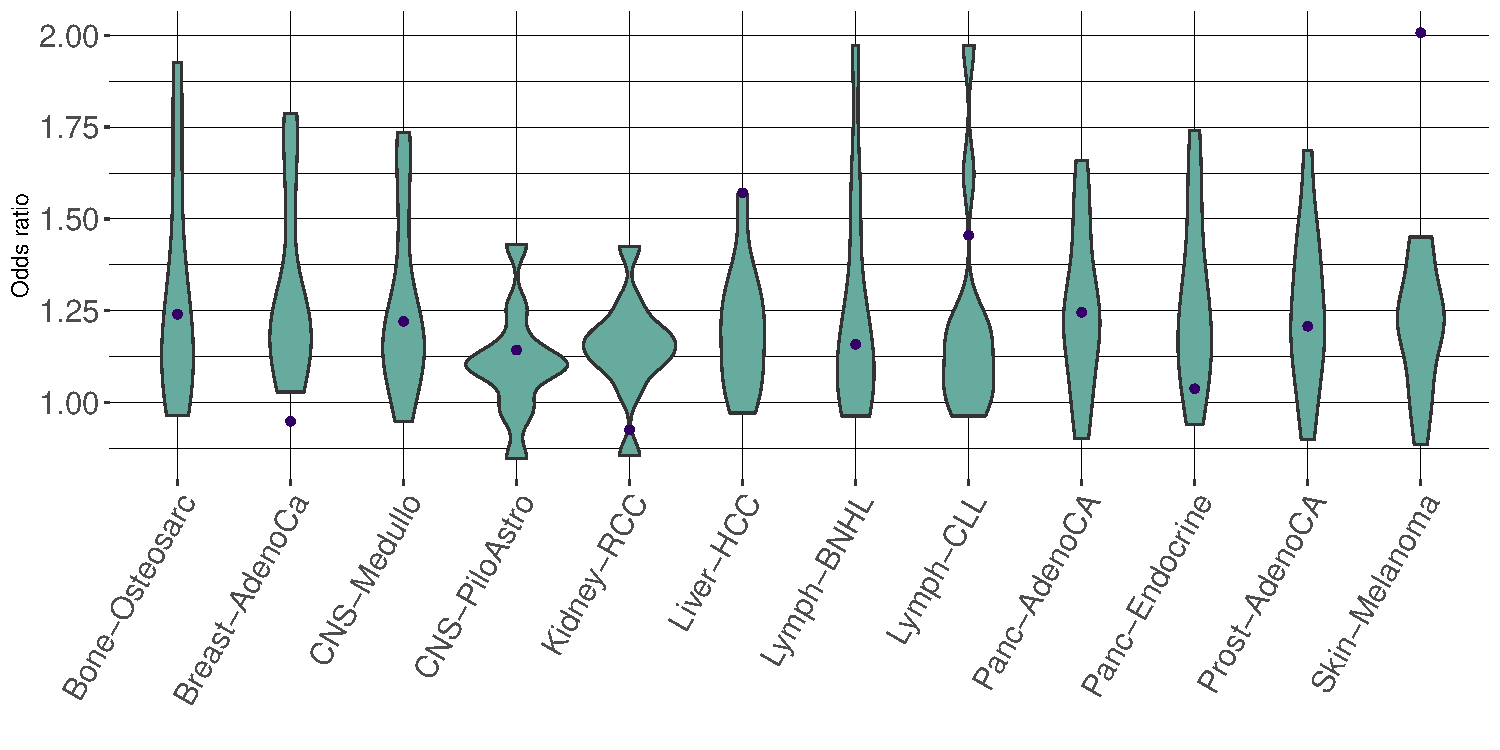
\includegraphics[scale=0.5]{graphics/mixed_or_violin.pdf}
    \caption{The impact of imbalanced DHS data on $OR$ is mild}
    \label{fig:mixed_or_violin}
    \end{subfigure} \\
    
    \vspace{0.3cm}
    \begin{subfigure}{\textwidth}
    \centering
    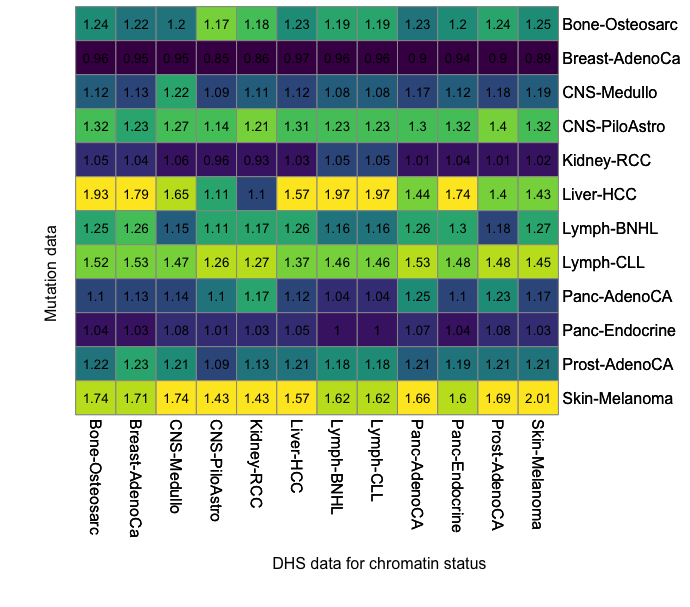
\includegraphics[scale=0.52]{graphics/mixed_or_heatmap.png}
    \caption{Chromatin structure is not discriminative of cancers}
    \label{fig:mixed_or_heatmap}
    \end{subfigure} 
\caption{}
    % \caption{\textbf{(a) The bias of mutations towards closed regions was not due to their large size compared to open regions but (b) this bias was unlikely the reason why GLE differs between cancers.} This figure shows an experiment where $OR$'s were calculated by cross-matching DHS data with mutation data of different cancers. In (a), the x-axis is the cancers whose DHS data was used, the y-axis is the distribution of $OR$ with mislabelled mutation data, with the purple dot indicating when mutation data of the correctly labelled cancer was used. In (b), the column labels are the cancers whose DHS data was used, the row labels are the cancers whose mutation data was used; each column is coloured by the rank of $OR$'s, brighter colours come from cancers whose mutation data produced the greater $OR$'s.}
    \label{fig:mixed_or}
\end{figure}